\section{Experimental Setup}
\label{sec:exp}


\begin{table*}[t]
    \footnotesize
    \centering
    \rowcolors{1}{white}{gray!10}
    \caption{\textbf{Experimental results on LoCoMo, LongMemEval, and HotpotQA datasets using F1-score (F1), LLM-as-a-Judge (Judge), and Cost under the \textit{performance-first} setting}.}
    \label{tab:exp_main}
    \begin{tabular}{lcccccccccccc}
        \toprule
        \rowcolor{white}
        \textbf{Methods} &
        \multicolumn{3}{c}{\textbf{LoCoMo}} &
        \multicolumn{3}{c}{\textbf{LongMemEval}} &
        \multicolumn{3}{c}{\textbf{HotpotQA}} &
        \multicolumn{3}{c}{\makecell[c]{\rowcolor{white}\textbf{Avg.}}} \\
        \cmidrule(lr){2-4} \cmidrule(lr){5-7} \cmidrule(lr){8-10} \cmidrule(lr){11-13}
        \rowcolor{white}
        & \textbf{F1} & \makecell[c]{\rowcolor{white}\textbf{Judge}} & \textbf{Cost$^\downarrow$}
        & \textbf{F1} & \makecell[c]{\rowcolor{white}\textbf{Judge}} & \textbf{Cost$^\downarrow$}
        & \textbf{F1} & \makecell[c]{\rowcolor{white}\textbf{Judge}} & \textbf{Cost$^\downarrow$}
        & \textbf{F1} & \makecell[c]{\rowcolor{white}\textbf{Judge}} & \textbf{Cost$^\downarrow$} \\
        \midrule
        \rowcolor{white}
        \multicolumn{13}{l}{\textbf{LLaMA-3.3-70B-Instruct}} \\
        ReadAgent & 22.48 & 31.05 & 0.57 & 20.75 & 27.72 & 13.68 & 15.33 & 30.08 & 4.19 & 19.52 & 29.62& 6.14 \\
        MemoryBank & 22.27 & 28.98 & 0.73 & 26.74 & 32.67 & 3.94 & 22.25 & 23.75 & 7.75 & 23.75 & 28.47 & 4.14 \\
        A-MEM & 26.43 & 32.96 & 2.88 & 21.74 & 33.17 & 80.02 & 43.25 & 54.69 & 26.74 & 30.47 & 40.27 & 32.07 \\
        LangMem & 22.31 & 25.96 & \textbf{0.48} & 12.00 & 17.00 & 16.60 & 22.78 & 22.66 & 10.95 & 19.03 & 21.87 & 9.34 \\
        Mem0 & 11.04 & 28.18 & 2.89 & 27.70 & 42.08 & 13.57 & 28.03 & 36.72& 4.30 & 22.26 & 35.66 & 6.92 \\
        MemoryOS & 30.62 & 34.55 & 1.97 & 12.97 & 33.50 & 38.83 & 34.50 & 43.36 & 13.32 & 26.03 & 37.14 & 18.04 \\
        LightMem & 33.88 & 40.76 & 1.50 & 26.74 & 48.51 &  5.28 & 45.73 & 58.37 & 10.10 & 35.45 & 49.21 & 5.63 \\
        \midrule
        \rowcolor{row-highlight}\textbf{BudgetMem-\textsc{Imp}} &
        38.75 & 50.32 & 1.80 &
        37.47 & 56.00 & 0.71 &
        49.31 & \textbf{65.77} & 1.35 &
        41.84 & 57.36 & \textbf{1.29} \\
        \rowcolor{row-highlight}\textbf{BudgetMem-\textsc{Rea}} &
        40.92 & 52.23 & 2.90 &
        \textbf{40.53} & 58.00 & \textbf{0.67} &
        51.12 & 61.93 & 0.99 &
        44.19 & 57.39 & 1.52 \\
        \rowcolor{row-highlight}\textbf{BudgetMem-\textsc{Cap}} &
        \textbf{43.05} & \textbf{54.62} & 2.40 &
        40.24 & \textbf{60.50} & 0.80 &
        \textbf{53.87} & 64.85 & \textbf{0.93} &
        \textbf{45.72} & \textbf{59.99} & 1.38 \\
        \midrule
        \rowcolor{white}
        \multicolumn{13}{l}{\textbf{Qwen3-Next-80B-A3B-Instruct}$^\dagger$} \\
        ReadAgent & 22.45 & 31.37 & 0.24 & 27.72 & 20.75 & 4.97 & 18.05 & 25.78 & 1.75 & 22.74 & 25.97& 2.32 \\
        MemoryBank & 23.53 & 34.71 & 0.25 & 10.56 & 28.22 & 3.45 & 18.64 & 31.25 & 1.79 & 17.58 & 31.39 & 1.83 \\
        A-MEM & 27.65 & 38.54 & 2.88 & 10.82 & 31.19 & 21.00 & 40.54 & 50.39 & 8.34 & 26.34& 40.04& 10.74\\
        LangMem & 20.89 & 23.40 & \textbf{0.14} & 11.01 & 14.00 & 3.99 & 20.77 & 21.09 & 17.56 & 17.56 & 19.50 & 2.82 \\
        Mem0 & 10.77 & 25.32 & 1.15 & 25.71 & 36.14 & 4.96 & 24.72 & 37.89 & 2.02 & 20.40 & 33.12 & 2.71 \\
        MemoryOS & 35.43 & 38.85 & 0.75 & 13.35 & 33.00 & 15.84 & 41.21 & 53.52 & 11.68 & 30.00 & 41.79 & 9.42 \\
        LightMem & 32.85 & 42.83 & 0.70 & 27.70 & 47.52 & 3.39 & 41.29 & 55.42 & 8.56& 33.95 & 48.59 & 4.21 \\
        \midrule
        \rowcolor{row-highlight}\textbf{BudgetMem-\textsc{Imp}} &
        40.14 & \textbf{54.38} & 0.80 &
        29.18 & 52.00 & 0.30 &
        46.67 & 57.42 & 0.63 &
        38.66 & 54.60 & 0.58 \\
        \rowcolor{row-highlight}\textbf{BudgetMem-\textsc{Rea}} &
        40.19 & 53.34 & 1.11 &
        \textbf{35.84} & \textbf{59.00} & 0.26 &
        57.67 & 70.83 & \textbf{0.17} &
        \textbf{44.57} & \textbf{61.06} & 0.51 \\
        \rowcolor{row-highlight}\textbf{BudgetMem-\textsc{Cap}} &
        \textbf{41.22} & 53.18 & 0.61 &
        31.01 & 56.00 & \textbf{0.17} &
        \textbf{58.70} & \textbf{72.08} & 0.22 &
        43.64 & 60.42 & \textbf{0.33} \\
        \bottomrule
        \rowcolor{white}\multicolumn{13}{l}{\small \textbf{Bold} indicates the best score within each base model block. Avg. is averaged over datasets for each metric.} \\
        \rowcolor{white}\multicolumn{13}{l}{
        \textbf{Cost} is computed by summing all tokens across model calls and applying the model’s respective input- and output-token prices}\\
        \rowcolor{white}\multicolumn{13}{l}{\small $^\dagger$ indicates no training using this base model (transfer evaluation only).} \\
    \end{tabular}
\end{table*}




\subsection{Datasets, Metrics, and Baselines}
\label{sec:datasets_metrics_baselines}

\paragraph{Datasets.}
We evaluate BudgetMem on three benchmarks that stress long-horizon memory and long-context question answering (QA): \textbf{LoCoMo}~\citep{maharana2024evaluating-locomo} and \textbf{LongMemEval}~\citep{wu2024longmemeval}, which are widely used for agent memory evaluation, and \textbf{HotpotQA}~\citep{yang2018hotpotqa}\footnote{we follow the evaluation protocol adopted in prior work~\citep{yu2025memagent}} as a representative long-context QA task. 


\paragraph{Metrics.}
We report both task performance and cost to characterize performance--cost trade-offs.
For task performance, we use F1-score (F1) and LLM-as-a-judge (Judge) to assess the correctness of a model prediction against the ground-truth answer.
For cost, we measure memory extraction cost by aggregating API usage (input \& output tokens) for all model calls made by BudgetMem during extraction, and converting token counts into monetary cost using the corresponding service pricing\footnote{\url{https://www.together.ai/pricing}}.



\paragraph{Baselines.}
We compare BudgetMem against a diverse set of strong memory-augmented baselines: 
(1) \textbf{ReadAgent}~\citep{lee2024human}, (2) \textbf{MemoryBank}~\citep{zhong2024memorybank}, (3) \textbf{A-MEM}~\citep{xu2025mem}, (4) \textbf{LangMem}~\citep{LangMem}, (5) \textbf{Mem0}~\citep{chhikara2025mem0}, (6) \textbf{MemoryOS}~\citep{kang2025memory}, and (7) \textbf{LightMem}~\citep{fang2025lightmem}. 
These baselines cover a broad range of memory architectures, providing a comprehensive comparison against prior agent memory systems. More details are provided in Appendix~\ref{appendix:imple_detail}.



\subsection{Implementation Details}
\label{sec:impl_details}


We use LLaMA-3.3-70B-Instruct~\citep{grattafiori2024llama} and Qwen3-Next-80B-A3B-Instruct~\citep{yang2025qwen3} as the base LLMs, accessed via an API service. 
We train the budget-tier router with LLaMA as the memory-extraction backbone, then directly test the same trained router with Qwen as the backbone without retraining.
For the retrieval and chunking, we split each history or document into fixed-length text chunks (with a default chunk size of 256 for LoCoMo and LongMemEval; 1024 for HotpotQA) and use Contriever~\citep{izacard2021unsupervised-contriever} as the default retriever. 
For each query, we retrieve a candidate set of chunks and then apply the same top-$K$ budget ($K{=}5$) for downstream memory processing, so that BudgetMem and all baselines operate under a matched retrieval context size.


As for training, we follow a $6/2/2$ split for train/validation/test across datasets, and keep the same data splits and evaluation protocols for all methods to ensure fair comparison.
% LR=?
We employ the Proximal Policy Optimization (PPO)~\citep{schulman2017proximal} as the default RL algorithm and use Adam optimizer with a batch size of 32 for up to 600 training steps.
Appendix~\ref{appendix:imple_detail} and~\ref{appendix:prompts} provide additional hyperparameters, prompts, and implementation details.




\begin{figure*}[t]
	\centering
	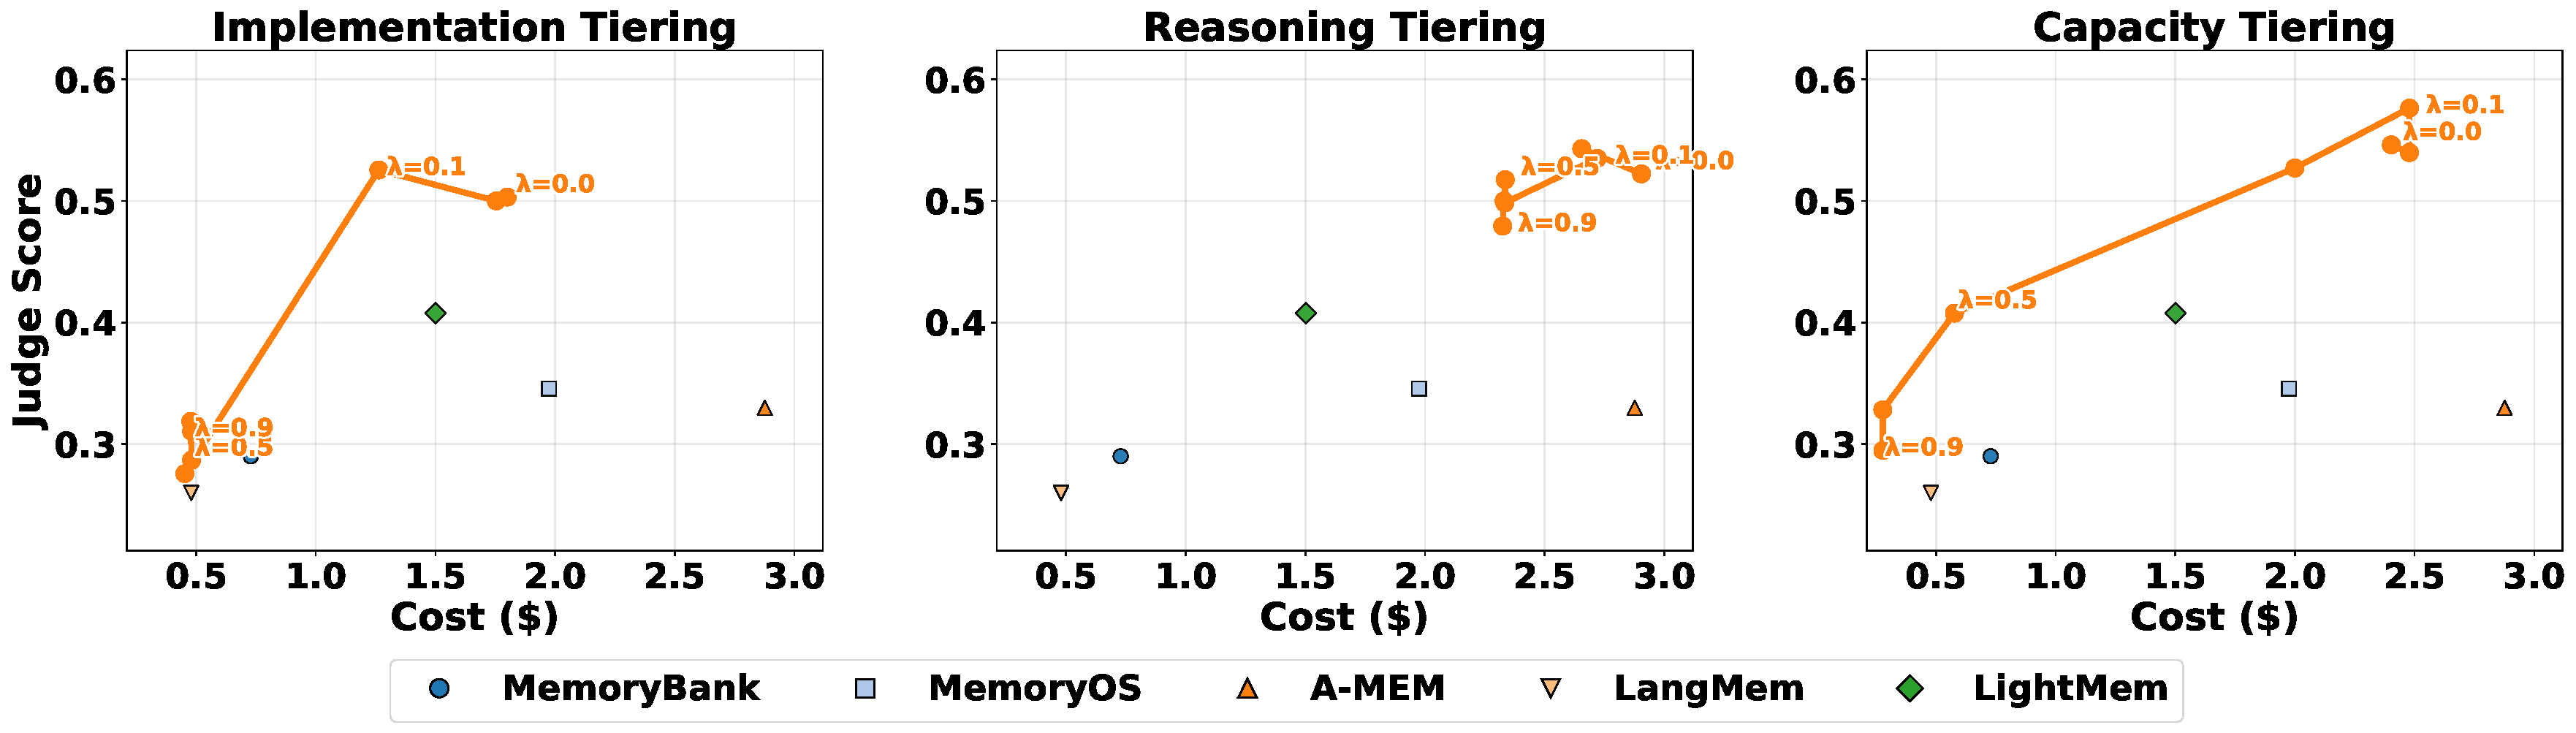
\includegraphics[width=1.0\linewidth]{figs/locomo_strategy_ABC.pdf}
        \caption{\textbf{Performance--cost trade-offs across tiering strategies on LoCoMo.} By varying the cost weight $\lambda$, BudgetMem traces smooth, controllable frontiers that shift toward higher performance as budget increases, and envelop baselines in both low- and high-cost regimes.}
	\label{Trade_off_Across_Tiering_Strategies}
\end{figure*}





\section{Experimental Analysis}
\label{sec:exp_analysis}



We organize experiments as follows. In Sec.~\ref{sec:main_results}, we report performance-first results ($\lambda=0$) and compare three variants: \textbf{BudgetMem-\textsc{Imp}}, \textbf{BudgetMem-\textsc{Rea}}, and \textbf{BudgetMem-\textsc{Cap}}. Sec.~\ref{sec:trade-off} varies $\lambda$ to trace performance--cost curves, Sec.~\ref{sec:ablation} ablates cost modeling and reward design, and Sec.~\ref{sec:discussion} provides further analysis.





\subsection{Main Results}
\label{sec:main_results}


As shown in Table \ref{tab:exp_main}, we evaluate BudgetMem under the performance-first setting on LoCoMo, LongMemEval, and HotpotQA, comparing against a diverse set of representative memory systems. The results support three key findings.

\textbf{Effectiveness.} BudgetMem delivers substantial improvements across all three datasets, consistently outperforming prior methods in both F1 and LLM-Judge. For example, on LongMemEval with the LLaMA-3.3-70B backbone, BudgetMem-\textsc{Cap} achieves a Judge score of 60.50, surpassing the strongest baseline LightMem (48.51) by a large margin, demonstrating stronger long-context evidence utilization and higher answer quality.



\textbf{Strong performance under controlled cost.} Even in the performance-first regime, BudgetMem remains cost-efficient, achieving higher quality without incurring excessive overhead. Notably, on HotpotQA with Qwen3-Next-80B-A3B, BudgetMem-\textsc{Cap} achieves the best Judge score (72.08) at a cost of 0.22, while BudgetMem-\textsc{Rea} reaches a comparable Judge score (70.83) at an even lower cost (0.17). This efficiency stems from BudgetMem's runtime, on-demand design: rather than processing the entire history offline, it retrieves query-relevant raw chunks and spends extraction compute only when needed. We note an exception on LoCoMo, where histories are shorter and offline pipelines incur less overhead, so cost differences across methods become less pronounced.


\textbf{Strongest overall performance on aggregate.}
When aggregating results across datasets, BudgetMem variants consistently rank at the top within each backbone block, indicating strong overall effectiveness rather than gains limited to a single benchmark. This trend holds for both LLaMA and Qwen, showing that BudgetMem delivers broadly strong performance across diverse evaluation settings under the performance-first regime.






\subsection{Exploring Trade-off Across Tiering Strategies}
\label{sec:trade-off}




As shown in Figure~\ref{Trade_off_Across_Tiering_Strategies}, we systematically compare the performance–cost distributions on LoCoMo across the three tiering axes. As the budget is relaxed (smaller $\lambda$), BudgetMem exhibits a smooth upward-leftward trend in the cost–performance, yielding a continuous and controllable trade-off frontier that envelopes prior baselines in both low- and high-cost regimes, achieving higher Judge at comparable cost or lower cost at comparable performance. Notably, \emph{implementation} and \emph{capacity} tiering span a broader cost range: implementation tiering delivers rapid Judge gains under moderate budgets, while capacity tiering continues to push the frontier outward as the budget increases, attaining the best quality in the high-budget regime. In contrast, \emph{reasoning} tiering exhibits pronounced cost concentration: because it primarily adjusts inference behaviors (e.g., direct/reflection) while holding the underlying model capacity fixed, the additional cost is dominated by a relatively stable token overhead, leading to a narrower spread in cost. This pattern suggests that the reasoning axis acts more like a fine-grained quality knob within a limited cost bandwidth, providing meaningful improvements at similar cost, but offering less room for exploring extremely low-budget settings or extrapolating to very high-budget performance than implementation/capacity tiering. Overall, BudgetMem consistently advances the Pareto frontier from budget-constrained to performance-first regimes, and the differences among tiering axes further indicate that implementation/capacity tiering is better suited for widening budget coverage and extrapolating the boundary, whereas reasoning tiering is most effective for refining quality within a relatively concentrated cost region.





\subsection{Ablating Reward-scale Alignment}
\label{sec:ablation}





As shown in Figure~\ref{Ablating_of_Reward_Scaling}, we ablate the reward-scale alignment (Sec.~\ref{sec:learn_routing}) under the capacity tiering strategy on LoCoMo. Because the task reward and cost reward can differ markedly in scale and variability, removing alignment makes optimization unstable and can bias learning toward the cost term, yielding a degenerate low-cost policy. Empirically, without reward-scale alignment (and with a cost weight $\lambda{=}0.3$), the router collapses to selecting the \textsc{Low} tier for most modules, substantially reducing answer quality and driving the Judge score to the lowest level. 
In contrast, with reward-scale alignment enabled, the router learns a more graded use of tiers, producing a much smoother and better-behaved performance--cost frontier.
This ablation highlights that reward-scale alignment is important for balancing learning signals, enabling meaningful cost--performance control rather than trivial cost minimization.



\begin{figure}[h]
	\centering
	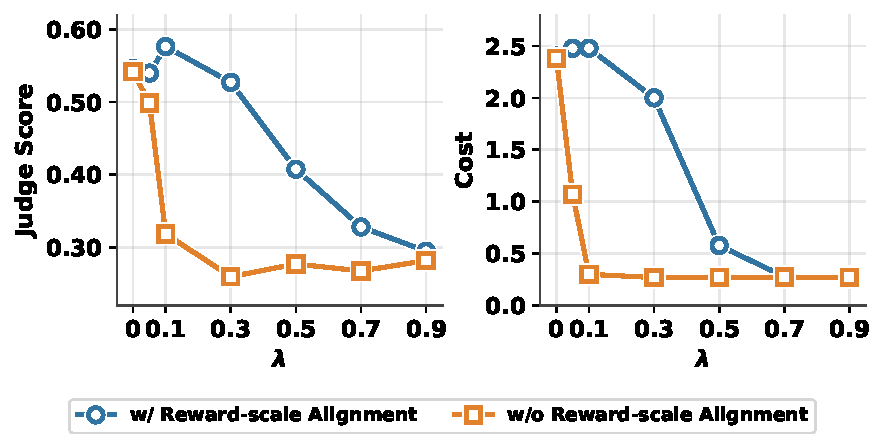
\includegraphics[width=1.0\linewidth]{figs/ablation_cost_reward_scaling.pdf}
        \caption{\textbf{Ablation of reward-scale alignment} under capacity tiering strategy on LoCoMo.}
	\label{Ablating_of_Reward_Scaling}
\end{figure}





\subsection{Discussion}
\label{sec:discussion}





\paragraph{Budget tier selection ratio.} Figure~\ref{Module_Ratio} analyzes module-level routing behavior on LongMemEval using the capacity tiering strategy by reporting the selection ratios of \textsc{Low}/\textsc{Mid}/\textsc{High} tiers under different cost weights $\lambda$. Overall, the router exhibits a clear and interpretable budget response: as cost pressure increases, it systematically shifts probability mass from higher-cost tiers to cheaper ones, providing module-level evidence that BudgetMem allocates computation in a cost-aware manner.

More concretely, with a small $\lambda$ (e.g., 0.1), the router assigns most modules to \textsc{Mid}, prioritizing quality. At $\lambda=0.3$, it increases the share of \textsc{Low} while maintaining a substantial \textsc{Mid} fraction, reflecting a controlled reduction in compute. Under larger $\lambda$, the policy further concentrates on \textsc{Low} across modules to meet stricter cost preferences. Overall, these trends confirm that BudgetMem modulates tier usage in a predictable way as the budget preference changes.




\begin{figure}[h]
	\centering
	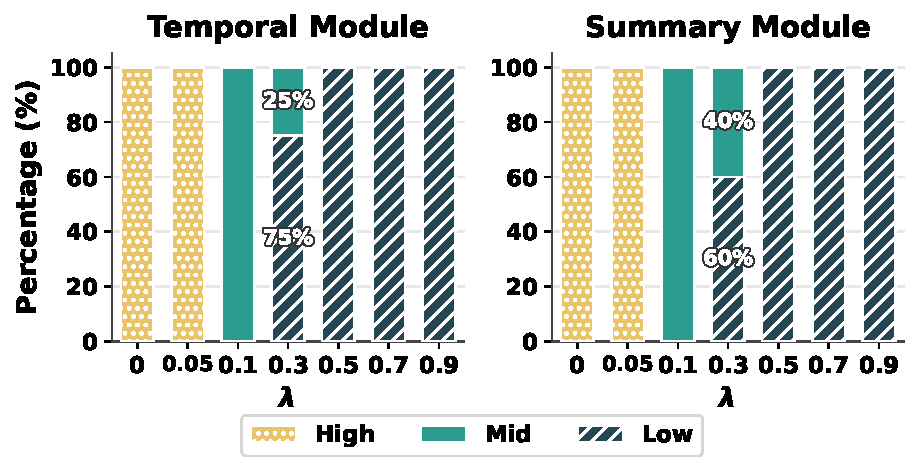
\includegraphics[width=1.0\linewidth]{figs/strategy_c_ratio_comparison.pdf}
        \caption{\textbf{Budget-tier selection ratios.} Module-wise \textsc{Low}/\textsc{Mid}/\textsc{High} routing ratios on LongMemEval under varying cost weights $\lambda$ using the capacity tiering strategy.}
	\label{Module_Ratio}
\end{figure}






\paragraph{Retrieval-size sensitivity analysis.} Figure~\ref{sensitivity_analysis} shows cost and Judge score as we vary the number of retrieved raw chunks on LoCoMo, evaluated under all three tiering strategies. Increasing the retrieval size predictably raises cost due to longer inputs and additional processing, and it often improves Judge score by providing more supporting evidence, reflecting the standard trade-off between evidence coverage and computational overhead.

However, the benefit is not monotonic. In our setting, retrieving 5 chunks provides the best balance between cost and quality. Retrieving too many chunks can degrade performance: additional chunks introduce more redundant or weakly relevant content, increasing noise and potentially distracting the LLM, which lowers Judge score. Conversely, retrieving too few chunks provides insufficient evidence and limits downstream gains. Overall, these results highlight retrieval size as an important practical knob for balancing evidence sufficiency against context noise and cost.




\begin{figure}[h]
	\centering
	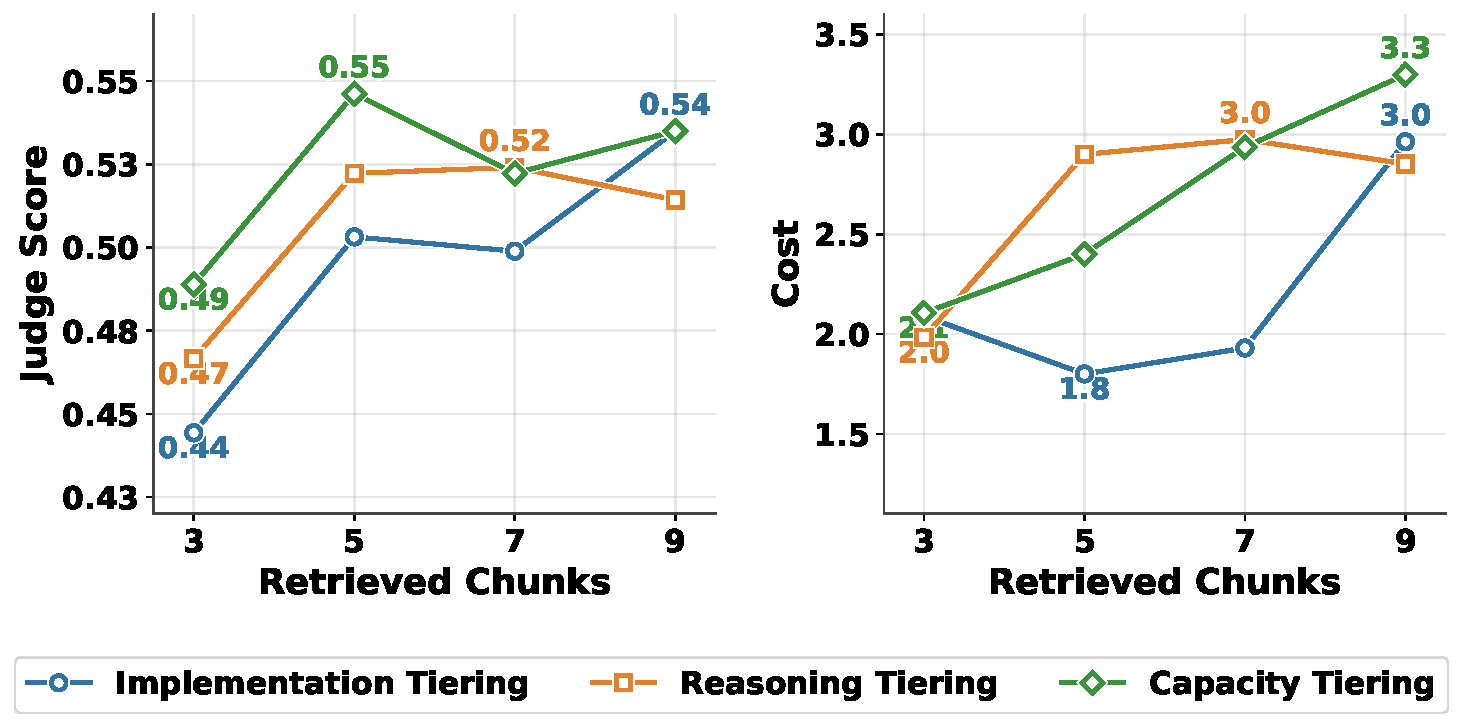
\includegraphics[width=1.0\linewidth]{figs/sensitivity_analysis.pdf}
        \caption{\textbf{Retrieval-size sensitivity on LoCoMo.} Cost and Judge versus the number of retrieved raw chunks, evaluated under all three tiering strategies.}
	\label{sensitivity_analysis}
    \vskip -0.1in
\end{figure}







\paragraph{Latency analysis.}
Although our main cost metric focuses on monetary cost, latency is also important for practical deployment. We therefore additionally measure latency under a controlled local deployment, using Qwen as the shared backbone and the same hardware and inference stack for all methods. We avoid API latency in this comparison because it can be strongly affected by network conditions and provider-side scheduling, making it less suitable for fair relative comparison. Tables~\ref{tab:latency_locomo_detail} and~\ref{tab:latency_locomo_batch} report absolute latency in this setting, while we mainly use them to compare relative pipeline overhead across methods.

As shown in Table~\ref{tab:latency_locomo_detail}, BudgetMem exhibits the expected latency trade-off under different budget settings. For implementation tiering, increasing the cost weight reduces total inference latency from 3881 ms at $\lambda=0$ to 1167 ms at $\lambda=0.9$, while the retrieval/filter latency drops from 1176 ms to 46 ms. Reasoning and capacity tiering also reduce latency, although the reduction is milder because their tiers mainly change inference behavior or model capacity rather than replacing the filtering implementation. In addition, the measured GPU time remains small, around 44--52 ms per query, indicating that the lightweight router itself introduces limited overhead. As shown in Table~\ref{tab:latency_locomo_batch}, all methods benefit from batching, and the relative overhead of BudgetMem remains broadly consistent across serving settings. Overall, these results indicate that the retrieval/filter overhead is practically controllable, while system-level acceleration of the full pipeline is orthogonal to our goal and left for future work.

\begin{table}[h]
    \centering
    \footnotesize
    % \setlength{\tabcolsep}{2.5pt}
    \caption{\textbf{Detailed latency on LoCoMo under controlled local deployment.}
    Batch size is 1. All values are in milliseconds. 
    \textbf{Off.} denotes average offline memory construction time, 
    \textbf{Total} denotes average total inference latency, 
    \textbf{Filt.} denotes average retrieval/filter module latency, and 
    \textbf{GPU} denotes average GPU time. 
    N/A indicates not applicable or not measured.}
    \label{tab:latency_locomo_detail}
    \begin{tabular}{@{}lrrrr@{}}
        \toprule
        \textbf{Method} & \textbf{Off.} & \textbf{Total} & \textbf{Filt.} & \textbf{GPU} \\
        \midrule
        MemoryOS & 40657 & 2842 & 1488 & N/A \\
        A-MEM    & 26842 & 1449 & 49   & N/A \\
        LightMem & 9740  & 1662 & 62   & N/A \\
        \midrule
        Ours-IMP ($\lambda=0$)   & N/A & 3881 & 1176 & 46 \\
        Ours-IMP ($\lambda=0.3$) & N/A & 2432 & 556  & 46 \\
        Ours-IMP ($\lambda=0.9$) & N/A & 1167 & 46   & 46 \\
        \midrule
        Ours-REA ($\lambda=0$)   & N/A & 3678 & 1274 & 47 \\
        Ours-REA ($\lambda=0.3$) & N/A & 3429 & 1216 & 45 \\
        Ours-REA ($\lambda=0.9$) & N/A & 3318 & 1209 & 48 \\
        \midrule
        Ours-CAP ($\lambda=0$)   & N/A & 3461 & 1228 & 44 \\
        Ours-CAP ($\lambda=0.3$) & N/A & 3058 & 1079 & 46 \\
        Ours-CAP ($\lambda=0.9$) & N/A & 2853 & 976  & 52 \\
        \bottomrule
    \end{tabular}
\end{table}


\begin{table}[h]
    \centering
    \footnotesize
    % \setlength{\tabcolsep}{3pt}
    \caption{\textbf{Batch-size scaling on LoCoMo.}
    We report average total inference latency under different batch sizes. 
    All values are in milliseconds. 
    \textbf{BS} denotes batch size. 
    For BudgetMem, we report Ours-REA with $\lambda=0$.}
    \label{tab:latency_locomo_batch}
    \begin{tabular}{@{}lrrrr@{}}
        \toprule
        \textbf{BS} & \textbf{MemoryOS} & \textbf{A-MEM} & \textbf{LightMem} & \textbf{Ours-REA} \\
        \midrule
        1  & 2842 & 1449 & 1662 & 3678 \\
        2  & 1633 & 845  & 1059 & 2295 \\
        4  & 974  & 518  & 775  & 1327 \\
        8  & 604  & 296  & 438  & 858  \\
        16 & 387  & 154  & 269  & 547  \\
        32 & 203  & 96   & 163  & 326  \\
        \bottomrule
    \end{tabular}
\end{table}